\documentclass[12pt]{amsart}
\usepackage{graphicx}
\usepackage{caption}
\usepackage{subcaption}
\usepackage[margin=1in]{geometry}
\pagestyle{empty}
\pagenumbering{gobble}
\usepackage{tipa}
\usepackage[colorlinks,allcolors=blue]{hyperref}

\renewcommand{\refname}{Selected References}
%\topmargin      =0.mm      % beyond 25.mm
%\oddsidemargin  =2.mm       % beyond 25.mm
%\evensidemargin =3.mm       % beyond 25.mm
%\headheight =0.mm \headsep    =0.mm \textheight =240.mm \textwidth=160.mm
\begin{document}
\title{ E\MakeLowercase{xploring} p\MakeLowercase{honetic} V\MakeLowercase{ariation} \MakeLowercase{in} u\MakeLowercase{nder}-r\MakeLowercase{esourced} l\MakeLowercase{anguages} u\MakeLowercase{sing} l\MakeLowercase{arge}-s\MakeLowercase{cale} d\MakeLowercase{ata} c\MakeLowercase{ollection}: A p\MakeLowercase{reliminary} l\MakeLowercase{ook} \MakeLowercase{at} G\MakeLowercase{eorgian} P\MakeLowercase{rosody} }
\maketitle

\vspace{-0.05in}

Due to the rising phenomenon of globalization, the need for developing language technologies for under-resourced languages has become more pressing. In this paper, we present methodology for low-resourced language documentation, and exemplify the usefulness of such techniques with a phonetic study of prosodic variability in Georgian, a Kartvelian agglutinative language spoken in the Caucasus Mountains of Eastern Europe. Used by 1.4 million speakers in the Republic of Georgia and members of the diaspora throughout the world, Georgian is an understudied language with very limited access to software and tools (e.g. spell checkers, electronic dictionaries and search engine tokenizers) which would facilitate its use in written form. While Georgian is the national language of Georgia, most computer systems sold in Georgia are offered in Russian or in English \cite{Sh}, and because most search engines lack support for Georgian, users perform internet searches using Russian or English keywords.

In 2014 we created open source libraries and tools to facilitate usage of the Georgian language by Georgian speakers \cite{Du}. One of these tools was Gismet, an Android application which can be used by Georgian speakers to train their Android smartphones to recognize their speech using PocketSphinx \cite{Hu}. The software was made freely available to the public and also open source on GitHub, a social coding site where developers can share and contribute to the source code.

Participants discover the application in the Google Play App Store. After installing it, they are led through a tutorial where they record 2-6 utterances to train the application to their voice. The stimuli consist of two SMS dictations, two web searches and two legal searches. Following the training phase, users can add additional training sentences or begin using the application anywhere in the Android system where keyboard input is provided. The training utterances are uploaded to a central server where they are processed using Praat and the CMUSphinx language model toolkit \cite{Wa} to customize the acoustic model for the speaker. The stimuli are comprised of six utterances which were elicited during fieldwork with three speakers in Batumi, Georgia.

Since 2014, over 1,000 users have used the application to train the default language model to their voices. The resulting dataset contains only elicited training recordings, similar to those obtained in an experimental setting. %, no user defined messages are included in the dataset.
The location of the participants is recorded via GPS technology, and informed consent for the anonymous analysis of their voices is provided voluntarily during the software installation process. This set-up enables us to conduct studies regarding various aspects of their speech production. Given the general lack of linguistic descriptions for spoken Georgian, the phonetic variation in the contemporaneous form of the language has not been studied, with very few exceptions \cite{Ch, CGB}.  For a first `case study' based on our corpus, we have selected prosodic variation, specifically the realization of pitch contour patterns in short utterances. The prosodic properties of Georgian are of particular interest, given the ability of its consonants to form extensive clusters \cite{Ch} combined with a phenomenon of vowel reduction. While the analysis of the entire corpus is underway, Figure 1 presents spectrograms of two speakers' production of the same short sentence, with distinct intonation contours. %To identify the existence of different prototypes, we apply a novel categorization tool based on the computation of similarity scores between intonation contours (following [4]).


\newpage
\begin{figure}
    \centering
        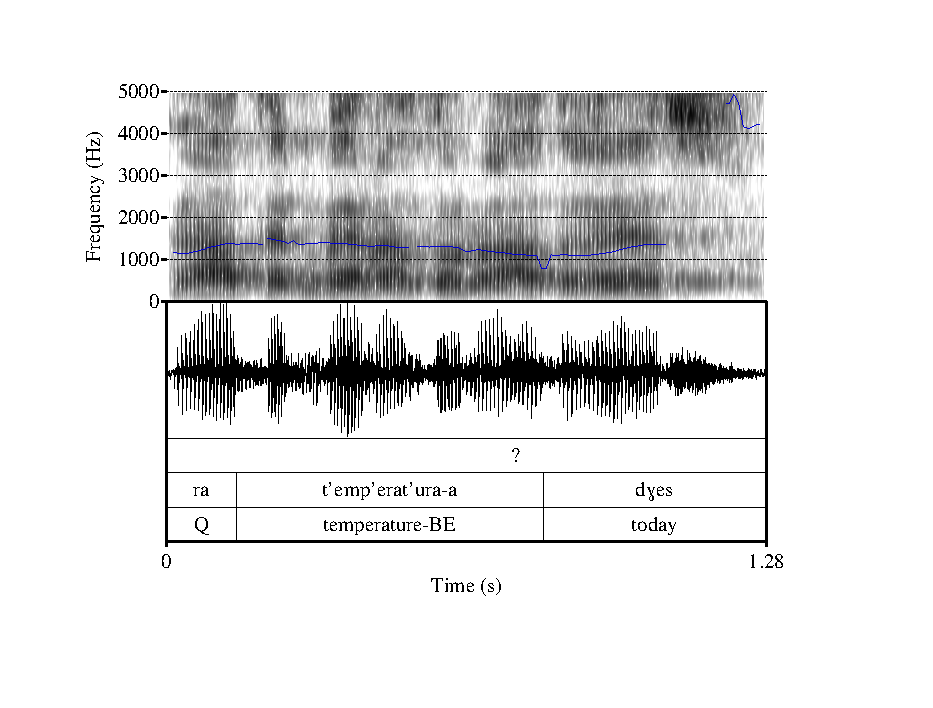
\includegraphics[scale=0.5]{prosody1}
        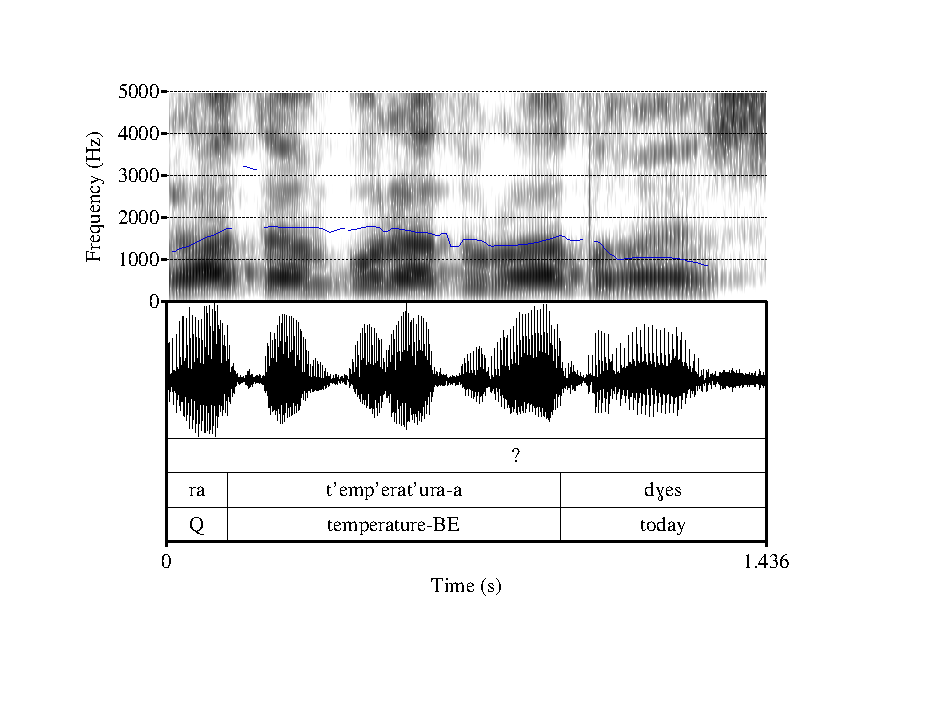
\includegraphics[scale=0.5]{prosody2}
    \caption{\footnotesize{\textit{\textsc{Left:} Spectrograms, pitch contours, waveforms and transcriptions of two male speakers' production of a short Georgian utterance with natural prosody}}}\label{fig:temp}
\end{figure}



\bibliographystyle{IEEEtran}

\begin{thebibliography}{17}

\bibitem[1]{Bo}Boersma, P. 2001. Praat, a system for doing phonetics by computer. \emph{Glot International} 5:9/10, 341--345.

\bibitem[2]{Ch}Chitoran, I. 1998. Georgian harmonic clusters: Phonetic cues to phonological representation. \emph{Phonology}, 15(2), 121-141.

\bibitem[3]{CGB}Chitoran, I., Goldstein, L. and Byrd, D. 2002. Gestural overlap and recoverability: Articulatory evidence from Georgian. \emph{Laboratory Phonology} 7, 419--447.

\bibitem[4]{Du}Dunham, J., Chiodo, G., \& Horner, J. 2014. LingSync \& the Online Linguistic Database: New Models for the Collection and Management of Data for Language Communities, Linguists and Language Learners. \emph{Proceedings of the 2014 Workshop on the Use of Computational Methods in the Study of Endangered Languages}, 1, 23--33.

\bibitem[5]{Ju}Juh{\'a}r, J., Sta{\v{s}}, J., \& Hl{\'a}dek, D. 2012. Recent progress in development of language model for Slovak large vocabulary continuous speech recognition. \emph{InTech: New technologies-trends, innovations and research}.


\bibitem[6]{Hu}Huggins-Daines, D., Kumar, M., Chan, A., Black, A.,  Ravishankar, M., \& Rudnicky,  A. I. 2006. PocketSphinx: A free, real-time continuous speech recognition system for hand-held devices. \emph{Proceedings of ICASSP}.


\bibitem[7]{Sh}Sherouse, P. 2014. Hazardous digits: Telephone keypads and Russian numbers in Tbilisi, Georgia. \emph{Language \& Communication}, 37, 1--11.


\bibitem[8]{Wa}Walker, W., Lamere, P., Kwok, P., Raj, B., Singh, R., Gouvea, E., Wolf, P. \& Woelfel, J. 2004. Sphinx-4: A flexible open source framework for speech recognition. \emph{Sun Microsystems, Inc}.


\end{thebibliography}

\end{document}
